\section{Track reconstruction}
\label{sec:track}

The track reconstruction in \lhcb is performed by several different algorithms~\cite{tracking}. In order to describe the process, it is first necessary to introduce the notion of track types and track states which are described in Sec.~\ref{sec:track:track-types} and Sec.~\ref{sec:track:track-states} respectively. Each of the tracking algorithms used in Run I are described in detail in Sec.~\ref{sec:track:algos} with special emphasis given to the upstream tracking algorithm. The duplicate track removal and track fit procedures are described in Sec.~\ref{sec:track:clone} and Sec.~\ref{sec:track:fit} respectively. Finally, the methods used to determine the performance of the track reconstruction using simulation are detailed in Sec.~\ref{sec:track:performance}.

\subsection{Track types}
\label{sec:track:track-types}

The tracks reconstructed in the \lhcb detector are divided into types depending on the sub-detectors in which they are reconstructed, as shown in Fig.~\ref{fig:track-types}. \velo tracks are defined as those which have measurements only in the \velo sub-detector. These tracks can be either forward or backward. Upstream tracks are defined as those which have measurements only in the \velo and TT (UT) sub-detectors. Upstream tracks are also referred to as \velott(\velout) tracks. T tracks are defined as those which have measurements solely in the T stations. Downstream tracks have measurements in the TT (UT) sub-detector and T stations. Long tracks have measurements in the \velo sub-detector and T stations and may also have measurements in the TT (UT) sub-detector. These tracks provide the best momentum resolution for particles which traverse the full tracking detector and are used in the majority of \lhcb analyses.

\begin{figure}[!tb]
\centering
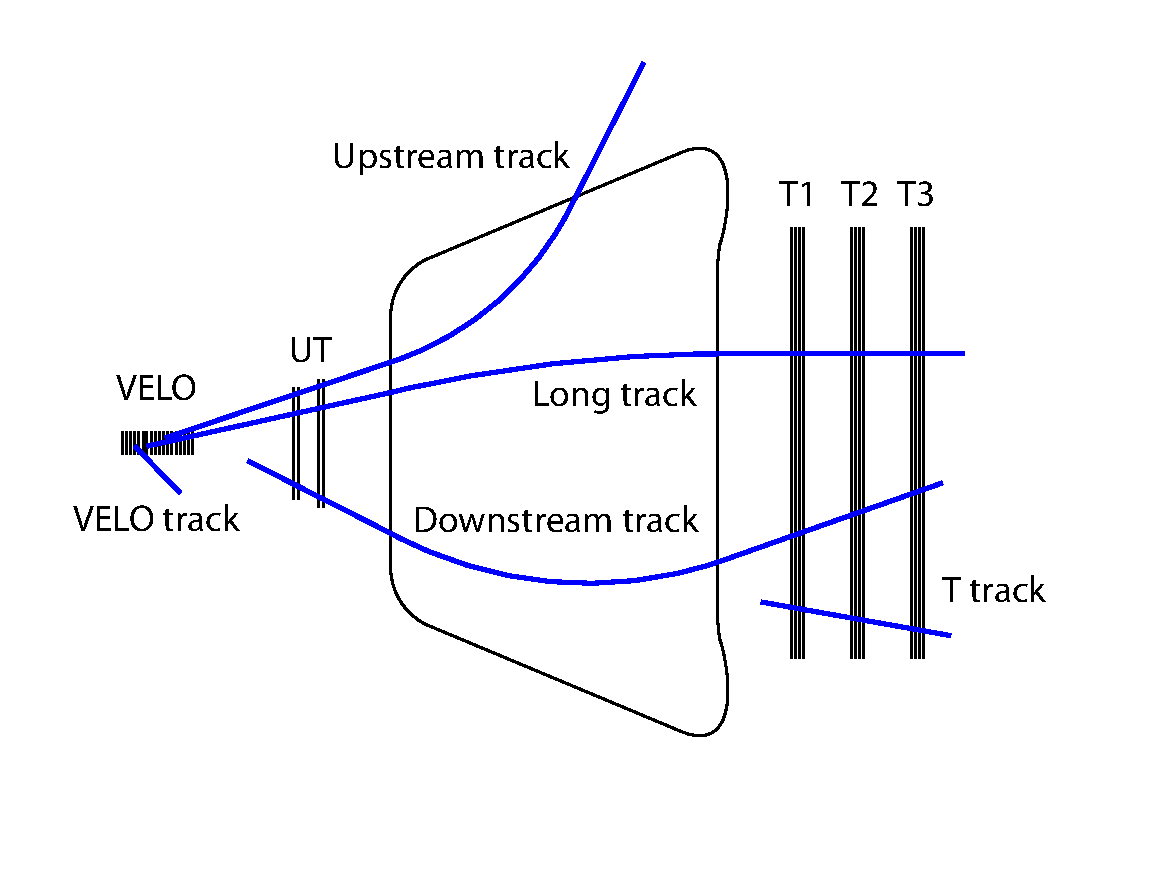
\includegraphics[width=0.8\textwidth]{figs/tracking/trackTypes.pdf}
\caption{Schematic diagram of the \lhcb tracking system. The various track types reconstructed by the different tracking algorithms are shown.}
\label{fig:track-types}
\end{figure}

\subsection{Track states}
\label{sec:track:track-states}

In \lhcb, a track is modelled as a series of straight line segments
called track states. A track state is defined by a state vector of the form

\begin{equation}
\vec x = 
\begin{pmatrix}
x \\
y \\
t_{x} \\
t_{y} \\
q/p \\
\end{pmatrix}
\text{with}~t_{x} = \frac{\partial x}{\partial z} ~\text{and}~ t_{y} = \frac{\partial y}{\partial z} 
\end{equation}

\noindent and a corresponding $5\times5$ state covariance matrix at a given position in $z$. Here, $q$ and $p$ are the charge and momentum of the track respectively.

\subsection{Track reconstruction algorithms}
\label{sec:track:algos}

In order to reconstruct the different track types, several tracking algorithms are employed. The two stand-alone algorithms, \velo tracking and track seeding, are described in Sec.~\ref{sec:track:algos:velo} and Sec.~\ref{sec:track:algos:seeding} respectively. The other algorithms use input from these two algorithms in order to perform a further track reconstruction.

\subsubsection{\velo tracking}
\label{sec:track:algos:velo}

The \velo tracking algorithm~\cite{fastvelo} is used to find tracks in the \velo. As there is no magnetic field in the \velo, tracks are expected to be approximately straight lines. The track search begins in the most downstream layer of the \velo. Quadruplets of hits are searched for in the $r$-sensors as shown in Fig.~\ref{fig:velo-tracking}. If they are found, they are extended back to smaller $z$ adding hits that are consistent with coming from the same track. Next, the same quadruplet search is performed for backward-going tracks. Triplets are then searched for, first backward-going and then forward-going, requiring that the hits have not been used in the quadruplet search.

Starting from the longest $r$-$z$ track, $\phi$ hits are searched for that are consistent with coming from the same track. These 3D tracks are then fitted with a $\chi^{2}$ minimization.

\begin{figure}[!tb]
  \centering
  \resizebox{\columnwidth}{!}{
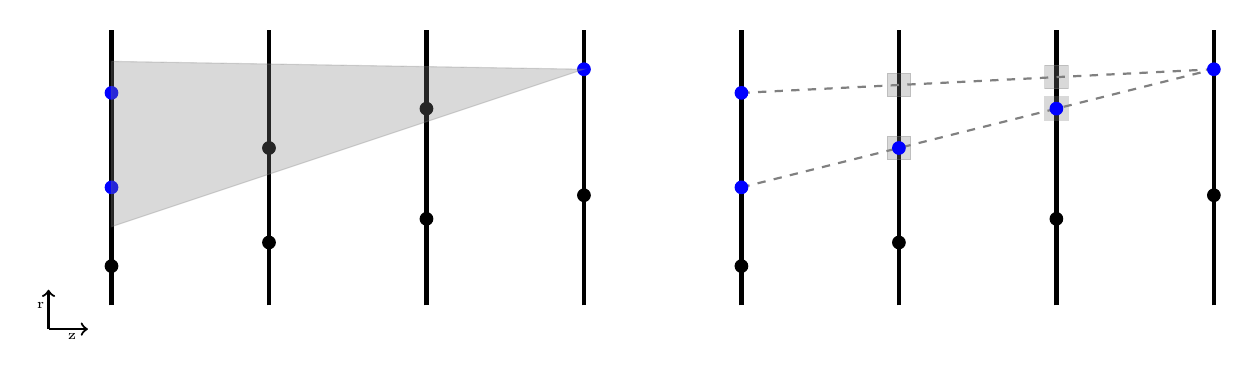
\begin{tikzpicture}
  %\draw[step=1cm,gray,very thin] (0,0) grid (15,4.5);
  \draw[ultra thick] (1.,0.5) -- (1.,4);
  \draw[ultra thick] (3,0.5) -- (3,4);
  \draw[ultra thick] (5,0.5) -- (5,4);
  \draw[ultra thick] (7,0.5) -- (7,4);
  
  \draw[fill,blue] (7,3.5) circle (0.08);
  \draw[fill,blue] (1,2) circle (0.08);
  \draw[fill] (3,2.5) circle (0.08);
  \draw[fill] (5,3) circle (0.08);
  
  \draw[fill] (1,1.) circle (0.08);
  \draw[fill] (3,1.3) circle (0.08);
  \draw[fill] (5,1.6) circle (0.08);
  \draw[fill] (7,1.9) circle (0.08);
  
  \draw[fill,blue] (1,3.2) circle (0.08);
  
  \draw[fill,gray,opacity=0.3] (7,3.5)--(1,1.5)--(1,3.6)--cycle;
  
  \draw[ultra thick] (9.,0.5) -- (9.,4);
  \draw[ultra thick] (11,0.5) -- (11,4);
  \draw[ultra thick] (13,0.5) -- (13,4);
  \draw[ultra thick] (15,0.5) -- (15,4);
  
  \draw[thick,gray, dashed] (9,2) -- (15,3.5);
  \draw[thick,gray, dashed] (9,3.2) -- (15,3.5);
  
  \draw[fill,gray,opacity=0.3] (10.85,2.35) rectangle (11.15,2.65);
  \draw[fill,gray,opacity=0.3] (12.85,2.85) rectangle (13.15,3.15);
  
  \draw[fill,gray,opacity=0.3] (10.85,3.15) rectangle (11.15,3.45);
  \draw[fill,gray,opacity=0.3] (12.85,3.25) rectangle (13.15,3.55);
  
  \draw[fill,blue] (15,3.5) circle (0.08);
  \draw[fill,blue] (9,2) circle (0.08);
  \draw[fill,blue] (11,2.5) circle (0.08);
  \draw[fill,blue] (13,3) circle (0.08);
  
  \draw[fill] (9,1.) circle (0.08);
  \draw[fill] (11,1.3) circle (0.08);
  \draw[fill] (13,1.6) circle (0.08);
  \draw[fill] (15,1.9) circle (0.08);
  
  \draw[fill,blue] (9,3.2) circle (0.08);
  
  \draw[thick,->] (0.2,0.2) -- (0.7,0.2);
  \draw[thick,->] (0.2,0.2) -- (0.2,0.7);
  
  \node[draw=none] at (0.5,0.1){\tiny z};
  \node[draw=none] at (0.1,0.5){\tiny r};
  
\end{tikzpicture}
}
  \caption{Quadruplets of hits are searched for in the \velo starting from the most downstream layer. Starting with a hit in that layer, a search window is opened in the fourth most downstream layer. From hits found within the window, the expected position of hits in the intermediate layers can be predicted assuming the track is a straight line in the $r$-$z$ projection. If hits fall within a tolerance of the expected positions, quadruplets are formed and a track is created.}
  \label{fig:velo-tracking}
\end{figure}

\subsubsection{Forward tracking}
\label{sec:track:algos:forward}

The Forward tracking algorithm~\cite{patforward} is used to find long tracks. A Hough transform is utilised to associate hits in the T-stations to each \velo track. The \velo track is linearly extrapolated to the T-stations and a symmetric search window is opened in each $x$ layer. The VELO track state and knowledge of the $\vec{B}$ field are used to project each selected hit to the $z$ position of a reference plane. Hits from the same particle are expected to be projected to the same $x$ position while random hits should be uniformly distributed. This procedure is shown schematically in Fig.~\ref{fig:forward-tracking}. The resulting clusters are fitted and outliers are removed using a $\chi^{2}$ criterium. An additional cluster search is used to add stereo hits that are consistent with the $x$-$z$ track. This 3D track is then fitted, outliers are removed and the best track candidate is chosen based on its $\chi^{2}$/dof.

\begin{figure}[!tb]
  \centering
  \resizebox{\columnwidth}{!}{
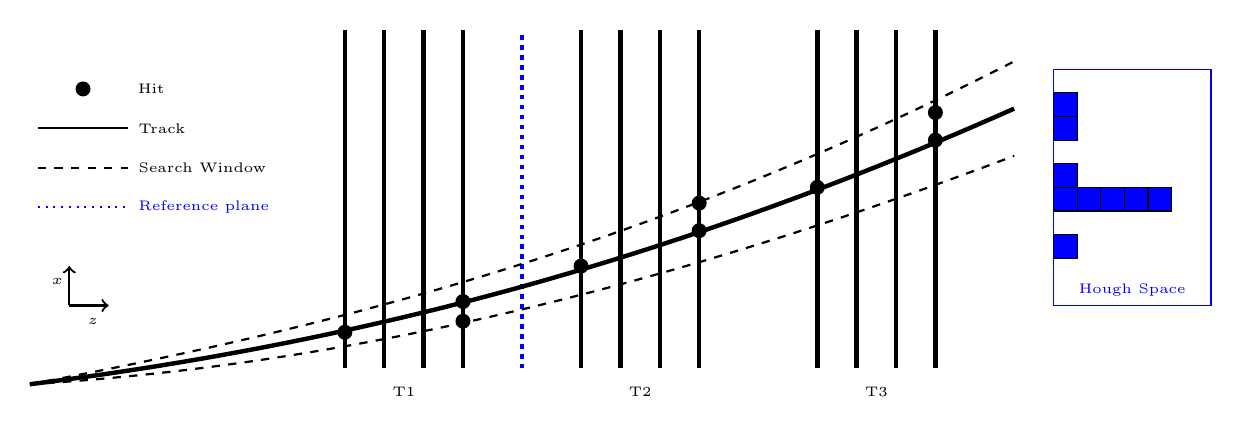
\begin{tikzpicture}
  %\draw[step=1cm,gray,very thin] (0,0) grid (15,5.);
    
  \draw[thick,->] (0.5,1) -- (0.5,1.5);
  \draw[thick,->] (0.5,1) -- (1.,1);
  \node[draw=none] at (0.35,1.3){\tiny $x$};
  \node[draw=none] at (0.8,0.8){\tiny $z$};
  
  \draw[ultra thick] (4,0.2) -- (4,4.5);
  \draw[ultra thick] (4.5,0.2) -- (4.5,4.5);
  \draw[ultra thick] (5,0.2) -- (5,4.5);
  \draw[ultra thick] (5.5,0.2) -- (5.5,4.5);

  \draw[ultra thick] (7,0.2) -- (7,4.5);
  \draw[ultra thick] (7.5,0.2) -- (7.5,4.5);
  \draw[ultra thick] (8,0.2) -- (8,4.5);
  \draw[ultra thick] (8.5,0.2) -- (8.5,4.5);

  \draw[ultra thick] (10,0.2) -- (10,4.5);
  \draw[ultra thick] (10.5,0.2) -- (10.5,4.5);
  \draw[ultra thick] (11,0.2) -- (11,4.5);
  \draw[ultra thick] (11.5,0.2) -- (11.5,4.5);

  \draw[dotted,blue,ultra thick] (6.25,0.2) -- (6.25,4.5);
  
  \draw[ultra thick] (0,0.0)  .. controls (4,0.5)  and (8,1.5) .. (12.5,3.5);
  \draw[thick,dashed] (0,0.0)  .. controls (4,0.25)  and (8,1.2) .. (12.5,2.9);
  \draw[thick,dashed] (0,0.0)  .. controls (4,0.75)  and (8,1.8) .. (12.5,4.1);
  
  \draw[fill] (4,0.66) circle [radius=2.5pt];
  \draw[fill] (5.5,1.05) circle [radius=2.5pt];

  \draw[fill] (7,1.5) circle [radius=2.5pt];
  \draw[fill] (8.5,1.95) circle [radius=2.5pt];

  \draw[fill] (10,2.5) circle [radius=2.5pt];
  \draw[fill] (11.5,3.1) circle [radius=2.5pt];

  \draw[fill] (5.5,0.8) circle [radius=2.5pt];
  \draw[fill] (8.5,2.3) circle [radius=2.5pt];
  \draw[fill] (11.5,3.45) circle [radius=2.5pt];
  
  \draw (13,1)[blue] rectangle (15,4);
  \node[draw=none,blue] at (14.0,1.2){\tiny Hough Space};
  \fill[blue,draw=black] (13,2.2) rectangle (13.3,2.5);
  \fill[blue,draw=black] (13.3,2.2) rectangle (13.6,2.5);
  \fill[blue,draw=black] (13.6,2.2) rectangle (13.9,2.5);
  \fill[blue,draw=black] (13.9,2.2) rectangle (14.2,2.5);
  \fill[blue,draw=black] (14.2,2.2) rectangle (14.5,2.5);
  \fill[blue,draw=black] (13.0,2.5) rectangle (13.3,2.8);
  

  \fill[blue,draw=black] (13,1.6) rectangle (13.3,1.9);
  
  \fill[blue,draw=black] (13.0,3.1) rectangle (13.3,3.4);
  \fill[blue,draw=black] (13,3.4) rectangle (13.3,3.7);
  
  \draw[white] (0.1,3.75) -- (1.25,3.75) node[anchor=west] {\tiny \textcolor{black}{Hit}};
  \draw[fill] (0.675,3.75) circle [radius=2.5pt];
  \draw[thick] (0.1,3.25) -- (1.25,3.25) node[anchor=west] {\tiny Track};
  \draw[thick,dashed] (0.1,2.75) -- (1.25,2.75) node[anchor=west] {\tiny Search Window};
  \draw[thick,dotted,blue,text opacity=1] (0.1,2.25) -- (1.25,2.25) node[anchor=west] {\tiny Reference plane};
  
  \node[draw=none] at (4.75,-0.1){\tiny T1};
  \node[draw=none] at (7.75,-0.1){\tiny T2};
  \node[draw=none] at (10.75,-0.1){\tiny T3};
  
\end{tikzpicture}
}
  \caption{A Hough transform is used to associate hits in the T-stations to a \velo track. Each hit within a search window around the extrapolated track is projected to the $z$ position of a reference plane. Hits from the same particle are expected to be projected to the same $x$ position while random hits should be uniformly distributed.}
  \label{fig:forward-tracking}
\end{figure}

\subsubsection{T seeding}
\label{sec:track:algos:seeding}

The T seeding algorithm~\cite{patseeding} is used to find T tracks. Track candidates are first searched for in the $x$-$z$ projection. A straight line is formed between suitable pairs of hits in T1 and T3. A compatible hit in T2 is added to form a parabola. Further hits in $x$ layers consistent with this parabola are added to the track candidate. A Hough transform is used to add stereo hits. A weighted least squares fit is then applied to each candidate.

\subsubsection{Track matching}
\label{sec:track:algos:match}

The track matching algorithm~\cite{patmatch} is also used to form long tracks. It takes both \velo and T tracks as input (seeds). The difference in $x$ and $y$ of the two seeds are calculated by extrapolating them both to the magnet bending plane ($\Delta x$) and the end of the T-stations ($\Delta y$) respectively. A matching criterion $\chi^{2}$ is formed using $\Delta x$, $\Delta y$, $\Delta t_{x}$ and $\Delta t_{y}$. If the track passes this criterion it is fitted and an estimate is made of its $q/p$.

\subsubsection{Downstream tracking}
\label{sec:track:algos:downstream}

The downstream tracking algorithm~\cite{patdownstream,sascha} forms downstream tracks. Each T track is extrapolated back to find the corresponding ($x$, $y$) point at the center of the magnet. A track estimate is formed using this point and the nominal interaction point. Hits in the TT consistent with the track estimate are selected. For each TT hit, a new track estimate is formed and consistent $x$ hits are collected. The collection of $x$ hits is fitted in the $x$-$z$ projection and outliers are removed. Stereo hits are added, the track is refitted and further outliers are removed. Finally, the best track candidate is chosen according to the number of hits it contains and the value of the $\chi^{2}$ from the fit.


\subsubsection{Upstream tracking}
\label{sec:track:algos:upstream}

The upstream tracking algorithm~\cite{patvelott} is used to find upstream tracks. These are generally low momentum tracks that will be bent out of acceptance by the magnet. It is executed at the end of the tracking sequence using \velo tracks which have not been upgraded to long tracks by any of the preceeding algorithms. 

Each \velo track is linearly extrapolated to the TT. Search windows are opened in each layer and the distance $\Delta x$ between the track and each hit is calculated. These $\Delta x$ values are scaled to a reference plane at the center of the TT. A Hough transform is utilised to associate the selected hits to the \velo track. Hits from the same particle are expected to be projected to the same $x$ position in the reference plane while random hits should be uniformly distributed. This procedure is shown schematically in Fig.~\ref{fig:velott-tracking}. An explicit assumption is made that every associated hit should lie on the same side of the extrapolated \velo track in the $x$-$z$ plane. 

 Each track candidate is fitted with a simplified $\chi^{2}$ minimisation and the $q/p$ of the track is estimated. Due to the fringe $\vec{B}$ field between the \velo and the TT a momentum estimate of $\delta p/p \sim~15\%$ is possible. The best track candidate is chosen based on the number of TT layers containing hits and the $\chi^{2}$ of the simplified fit. Each of the \velott tracks is subsequently fitted with a Kalman filter, described in Sec.~\ref{sec:track:fit}, in order to obtain the most accurate estimates of track parameters along with their corresponding covariances.

\begin{figure}[!tb]
  \centering
  \resizebox{\columnwidth}{!}{
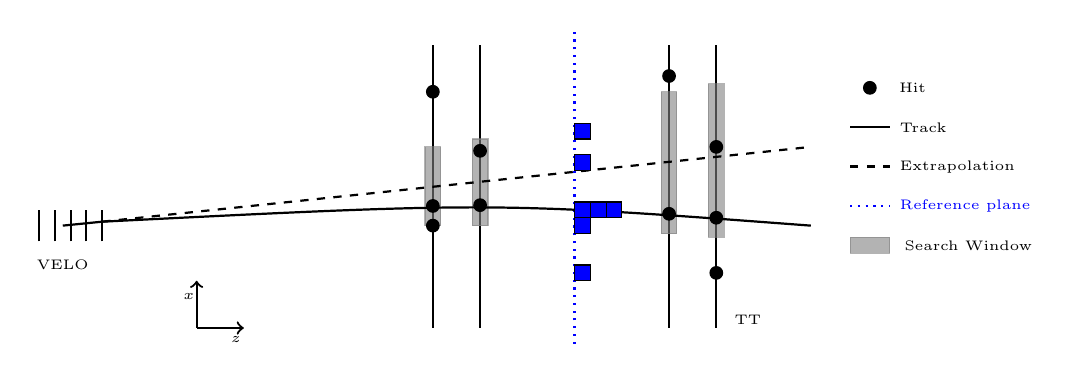
\begin{tikzpicture}
  %\draw[step=1cm,gray,very thin] (0,0) grid (13,4);

  \draw[thick,->] (2.2,0.2) -- (2.2,0.8);
  \draw[thick,->] (2.2,0.2) -- (2.8,0.2);
  \node[draw=none] at (2.1,0.6){\tiny $x$};
  \node[draw=none] at (2.7,0.05){\tiny $z$};

  \draw[thick] (0.2,1.3) -- (0.2,1.7);
  \draw[thick] (0.4,1.3) -- (0.4,1.7);
  \draw[thick] (0.6,1.3) -- (0.6,1.7);
  \draw[thick] (0.8,1.3) -- (0.8,1.7);
  \draw[thick] (1.0,1.3) -- (1,1.7);

  \draw[thick] (5.2,0.2) -- (5.2,3.8);
  \draw[thick] (5.8,0.2) -- (5.8,3.8);
  \draw[thick] (8.2,0.2) -- (8.2,3.8);
  \draw[thick] (8.8,0.2) -- (8.8,3.8);

  \draw[thick,dotted,blue] (7,0) -- (7,4);

  \draw[fill,gray,opacity=0.6] (5.1,1.5) rectangle (5.3,2.5);
  \draw[fill,gray,opacity=0.6] (5.7,1.5) rectangle (5.9,2.6);
  \draw[fill,gray,opacity=0.6] (8.1,1.4) rectangle (8.3,3.2);
  \draw[fill,gray,opacity=0.6] (8.7,1.35) rectangle (8.9,3.3);
  
  \draw[thick] (0.5,1.5) -- (1,1.5+0.5*0.1);
  \draw[thick,dashed] (1,1.5+0.5*0.1) -- (10,1.5+10*0.1);
  \draw[thick] (1,1.5+0.5*0.1) .. controls (6,1.8) .. (10,1.5);

  \draw[fill] (5.2,1.75) circle (0.08);
  \draw[fill] (5.8,1.76) circle (0.08);
  \draw[fill] (8.2,1.65) circle (0.08);
  \draw[fill] (8.8,1.6) circle (0.08);

  \draw[fill] (5.2,1.5) circle (0.08);
  \draw[fill] (5.2,3.2) circle (0.08);
  \draw[fill] (5.8,2.45) circle (0.08);
  \draw[fill] (8.2,3.4) circle (0.08);
  \draw[fill] (8.8,2.5) circle (0.08);
  \draw[fill] (8.8,0.9) circle (0.08);

  \fill[blue,draw=black] (7.0,1.6) rectangle (7.2,1.8);
  \fill[blue,draw=black] (7.2,1.6) rectangle (7.4,1.8);
  \fill[blue,draw=black] (7.4,1.6) rectangle (7.6,1.8);
  \fill[blue,draw=black] (7.0,1.4) rectangle (7.2,1.6);

  \fill[blue,draw=black] (7.0,0.8) rectangle (7.2,1.);
  \fill[blue,draw=black] (7.0,2.2) rectangle (7.2,2.4);
  \fill[blue,draw=black] (7.0,2.6) rectangle (7.2,2.8);

  \node[draw=none] at (0.5,1){\tiny VELO};
  \node[draw=none] at (9.2,0.3){\tiny TT};

  %\draw[thick] (10.5,3.25) -- (11.,3.25)  node[anchor=west] {\tiny Track};
  %\draw[fill] (11.,3.25) circle [radius=2pt]  node[anchor=west] {\tiny Hit};
  \draw[white] (10.5,3.25) -- (11.,3.25)  node[anchor=west] {\tiny \textcolor{black}{Hit}};
  \draw[fill] (10.75,3.25) circle (0.08);
  \draw[thick] (10.5,2.75) -- (11.,2.75)  node[anchor=west] {\tiny Track};
  \draw[thick,dashed] (10.5,2.25) -- (11.,2.25)  node[anchor=west] {\tiny Extrapolation};
  \draw[thick,dotted,blue] (10.5,1.75) -- (11.,1.75)  node[anchor=west] {\tiny Reference plane};
  \draw[fill,gray,opacity=0.6] (10.5,1.15) rectangle (11.0,1.35);
  \node[draw=none] at (12.0,1.25){\tiny Search Window};
\end{tikzpicture}
}

  \caption{A Hough transform is utilised to associate the selected TT hits to the \velo track. Hits from the same particle are expected to be projected to the same $x$ position in the reference plane while random hits should be uniformly distributed.}
  \label{fig:velott-tracking}
\end{figure}

\subsection{Clone removal}
\label{sec:track:clone}

As there are two independent algorithms to produce long tracks and several track types are subtracks of other types, it is necessary to avoid or remove duplicate tracks found by multiple algorithms. This is accounted for in two different ways. Some algorithms are only allowed to use tracks or hits that have not been previously used. When there is a significant overlap of hits between two tracks, the track with the smaller number of hits is discarded. 

\subsection{Track fit}
\label{sec:track:fit}

The purpose of the track fit  is to obtain the most accurate estimates of track parameters along with their corresponding covariances. Track parameters are used to match to particle identification objects (e.g. Cherenkov rings), find primary and secondary vertices and calculate the kinematics and invariant masses of particle combinations. The track $\chi^{2}$ is used to select good quality tracks. 

A Kalman filter is used to fit the tracks. With this approach, multiple scattering is taken into account as process noise and corrections due to energy losses are applied~\cite{kalman}. The transport through the magnetic field is evaluated using a Runge-Kutta method. The propagation and projection functions are linearised around a reference track state using a Taylor expansion~\cite{jeroen}.

Track candidates can be considered as a collection of track states (initially provided by the individual tracking algorithms) and measurements (tracking station hits). The Kalman filter can be divided into two steps, shown schematically in Fig.~\ref{fig:kalman}. Firstly, the parameters of a state at $z_{k}$ are predicted given a state at $z_{k-1}$. Next, the state at $z_{k}$ is updated with information of the measurement at this position. These two steps are repeated until all the measurements have been added. In \lhcb the filter is run in both the forward and the backward directions and the average is taken for smoothing.

\begin{figure}[!tb]
  \centering
  \resizebox{\columnwidth}{!}{
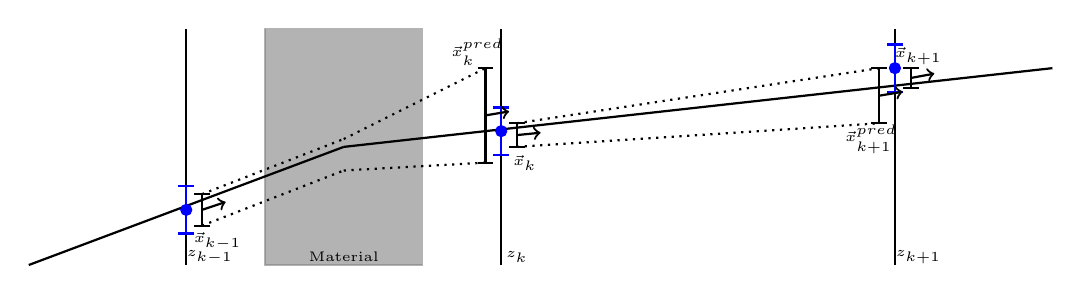
\begin{tikzpicture}
  %\draw[step=1cm,gray,very thin] (0,0) grid (14,3);
  
  \draw[fill,gray,opacity=0.6] (3,0) rectangle (5,3);
  
  \draw[thick] (2,0) -- (2,3);
  \draw[thick] (6,0) -- (6,3);
  \draw[thick] (11,0) -- (11,3);

  \draw[thick] (0,0.) -- (4,1.5);
  \draw[thick] (4,1.5) -- (13,2.5);

  %point 1
  \draw[fill,blue] (2,0.7) circle [radius=2pt];
  \draw[thick,blue] (2,0.4) -- (2,1.);
  \draw[thick,blue] (1.9,0.4) -- (2.1,0.4);
  \draw[thick,blue] (1.9,1.) -- (2.1,1.);

  %point 2
  \draw[fill,blue] (6,1.7) circle [radius=2pt];
  \draw[thick,blue] (6,1.4) -- (6,2.);
  \draw[thick,blue] (5.9,1.4) -- (6.1,1.4);
  \draw[thick,blue] (5.9,2.) -- (6.1,2.);

  %point 3
  \draw[fill,blue] (11,2.5) circle [radius=2pt];
  \draw[thick,blue] (11,2.2) -- (11,2.8);
  \draw[thick,blue] (10.9,2.2) -- (11.1,2.2);
  \draw[thick,blue] (10.9,2.8) -- (11.1,2.8);

  %state 1
  \draw[thick] (2.2,0.5) -- (2.2,0.9);
  \draw[thick] (2.1,0.5) -- (2.3,0.5);
  \draw[thick] (2.1,0.9) -- (2.3,0.9);
  \draw[thick,->] (2.2,0.7) -- (2.5,0.8);

  % state 2 pred
  \draw[thick] (5.8,1.3) -- (5.8,2.5);
  \draw[thick] (5.7,1.3) -- (5.9,1.3);
  \draw[thick] (5.7,2.5) -- (5.9,2.5);
  \draw[thick,->] (5.8,1.9) -- (6.1,1.95);

  % state 2 
  \draw[thick] (6.2,1.5) -- (6.2,1.8);
  \draw[thick] (6.1,1.5) -- (6.3,1.5);
  \draw[thick] (6.3,1.8) -- (6.1,1.8);
  \draw[thick,->] (6.2,1.65) -- (6.5,1.68);

  % state 3 pred 
  \draw[thick] (10.8,1.8) -- (10.8,2.5);
  \draw[thick] (10.7,1.8) -- (10.9,1.8);
  \draw[thick] (10.7,2.5) -- (10.9,2.5);
  \draw[thick,->] (10.8,2.15) -- (11.1,2.2);

  % state 3 
  \draw[thick] (11.2,2.25) -- (11.2,2.5);
  \draw[thick] (11.1,2.25) -- (11.3,2.25);
  \draw[thick] (11.1,2.5) -- (11.3,2.5);
  \draw[thick,->] (11.2,2.375) -- (11.5,2.43);

  \draw[thick,dotted] (2.2,0.9) -- (4,1.6);
  \draw[thick,dotted] (2.2,0.5) -- (4,1.2);
  \draw[thick,dotted] (4,1.6) -- (5.8,2.5);
  \draw[thick,dotted] (4,1.2) -- (5.8,1.3);
  \draw[thick,dotted] (6.2,1.8) -- (10.8,2.5);
  \draw[thick,dotted] (6.2,1.5) -- (10.8,1.8);

  \node[draw=none] at (2.3,0.1){\tiny $z_{k-1}$};
  \node[draw=none] at (6.2,0.1){\tiny $z_{k}$};
  \node[draw=none] at (11.3,0.1){\tiny $z_{k+1}$};

  \node[draw=none] at (2.4,0.3){\tiny $\vec{x}_{k-1}$};
  \node[draw=none] at (5.7,2.7){\tiny $\vec{x}_{k}^{pred}$};
  \node[draw=none] at (6.3,1.3){\tiny $\vec{x}_{k}$};
  \node[draw=none] at (10.7,1.6){\tiny $\vec{x}_{k+1}^{pred}$};
  \node[draw=none] at (11.3,2.65){\tiny $\vec{x}_{k+1}$};

  \node[draw=none] at (4,0.1){\tiny Material};
        
    \end{tikzpicture}
}
  \caption{A schematic diagram of the Kalman filter showing the prediction of a state $z_{k}$ given a state at $z_{k-1}$. The state is at $z_{k}$ is subsequently updated with information of the measurement at this position. This process is repeated until all measurements have been added.}
  \label{fig:kalman}
\end{figure}

\subsection{Tracking performance}
\label{sec:track:performance}

The figures of merit used to evaluate the performance of tracking algorithms are the reconstruction efficiency, ghost rate and execution time and are determined using simulated events. The simulated samples used in the following sections to benchmark the performance of the upstream tracking algorithms for both the \lhcb Upgrade and \lhcb Run II are shown in Table~\ref{tab:track-mc-samples}.

\begin{table}[!tb]
\caption{The simulated samples used in the following sections to benchmark the performance of the upstream tracking algorithms for both the \lhcb Upgrade and \lhcb Run II.}
\begin{center}
\begin{tabular}{c|c|c|c|c}
  & Decay Mode & $\sqrt{s}$~[\tev] & $\nu$ & Bunch spacing~[\ns] \\ 
  \hline
  Run II & \BsToPhiPhi, min. bias & 13 & 1.9 & 25 \\
  Upgrade & \BdToKstmm, min. bias & 14 & 7.6 & 25 \\
  \end{tabular}
\end{center}
\label{tab:track-mc-samples}
\end{table}

\subsubsection{Reconstruction efficiency}
\label{sec:track:eff}
The reconstruction efficiency is measured by comparing the number of correctly reconstructed tracks with the number of tracks defined to be reconstructible. This is made possible using truth information available in simulated samples. Within the \lhcb framework the following definitions are used:

\begin{itemize}

\item A particle is reconstructible as a \velo track if there are hits associated to it in at least three $r$ and three $\phi$ \velo sensors.

\item A particle is reconstructible as a long track if it fulfils the requirements to be reconstructible in both the \velo sub-detector and the T stations.

\item A particle is considered reconstructed if at least 70\% of both the \velo and T station hits on a track are associated to it and the track has no more than 1 wrongly associated TT (UT) hit.

\end{itemize}

\noindent The reconstruction efficiency is defined as

\begin{equation}
\epsilon_{rec} = \frac{N_{\text{reconstructible~and~reconstructed}}}{N_{\text{reconstructible}}}.
\end{equation}

When calculating the efficiency of the \velott (\velout) algorithm itself, particles are required to be reconstructible as a long track, have been correctly reconstructed in the \velo and have a matched TT (UT) hit in at least 3 TT (UT) layers. 

When considering the effect of using \velott (\velout) tracks as input to the Forward algorithm, no requirement is made that the particle has associated TT (UT) hits or has been correctly reconstructed in the \velo. Therefore, any inefficiency contains contributions from both the \velott (\velout) algorithm and the acceptance of the TT (UT) detector. 

In this note, further requirements are made to both the numerator and the denominator:

\begin{itemize}
\item The particle is required not to be an electron.
\item The pseudorapidity of the particle must lie between 2 and 5.
\item The particle is required to be \bquark-hadron daughter.
\item The particle must have \pt\textgreater~0.5\gevc.
\end{itemize}


\subsubsection{Ghost rate and clone tracks}
\label{sec:track:gr}
A ghost track is a track that has no matching simulated particle. The ghost rate is defined as

\begin{equation}
\text{Ghost rate}  = \frac{N_{\text{ghost~tracks}}}{N_{\text{tracks}}}.
\end{equation}

\noindent In all cases the following requirements are applied to both the numerator and denominator:

\begin{itemize}
\item The pseudorapidity of the track must lie between 2 and 5.
\item Tracks are required to have \pt\textgreater~0.5\gevc.
\end{itemize}

A track matched to a simulated particle with at least one other associated track is said to be a clone.

\subsubsection{Execution time}
\label{sec:track:timing}

The execution time of the individual algorithms is measured by the \lhcb event reconstruction application, \brunel. As the timing is machine dependent, the same machine is used for each measurement to facilitate direct comparisons. A simulated ``minimum bias'' sample is used in order to not give undue weight to a certain kind of event.

